\documentclass[draft,grl]{agutex}
%\documentclass[agums,grl]{agutex}

%% -----------------------
% COMMENT PRIOR SUBMISSION

%\usepackage{xcolor}
%\usepackage[letterpaper]{geometry}
%\usepackage{draftwatermark}
%\SetWatermarkText{Draft}
%\SetWatermarkScale{5}

%% -----------------------

\usepackage{graphicx}
\graphicspath{ {figures/} }

\usepackage{lineno}
\linenumbers*[1]
%\setlength{\columnsep}{25pt}
% KMS: Added more separation between the columns for better readability

% -----------------------


\authorrunninghead{GRIMA ET AL.}

\begin{document}

\titlerunninghead{BRINE EXTENT AT MCMURDO ICE SHELF}

\authoraddr{Corresponding author: C. Grima,
Institute for Geophysics, J.J. Pickle Research Campus, Bldg. 196, 10100 Burnet Rd. (R2200), Austin, TX 78758-4445, USA
(cyril.grima@gmail.com)}


%% ------------------------------------------------------------------------ %%
%
%  TITLE
%
%% ------------------------------------------------------------------------ %%


\title{Radar detection of the brine extent at McMurdo Ice Shelf, Antarctica, and its control by snow accumulation}

%% ------------------------------------------------------------------------ %%
%
%  AUTHORS AND AFFILIATIONS
%
%% ------------------------------------------------------------------------ %%

\authors{Cyril Grima,\altaffilmark{1}
Jamin S. Greenbaum,\altaffilmark{1} Erika J. Lopez Garcia,\altaffilmark{1}
Krista M. Soderlund,\altaffilmark{1} Arami Rosales,\altaffilmark{1,2}
Donald D. Blankenship,\altaffilmark{1} and Duncan A. Young\altaffilmark{1}}

\altaffiltext{1}{Institute for Geophysics, University of Texas at Austin, TX 78758, USA.}
\altaffiltext{2}{Department of Physics, University of Texas at Austin, TX 78712, USA.}

%% ------------------------------------------------------------------------ %%
%
%  ABSTRACT
%
%% ------------------------------------------------------------------------ %%

\begin{abstract}
We derive the surface density and brine infiltration depth/extent at McMurdo Ice Shelf, Antarctica, from combined analysis of radar profiles and radar statistical reconnaissance of the surface from 2011-2012 austral summer airborne observations. Most of the brine boundaries appear controlled, directly or indirectly, by the snow accumulation pattern. The infiltration is bounded westward by an ablation area and resides just above the pore close-off depth over most of its extent. The eastern brine limit matches a light-snow corridor, suggesting a reversed pressure gradient at depth that might sharply slow down the infiltration. Brine into ice is confirmed at the deepest locations north and east of Williams Field. The ice-ocean interface is undetected west of the infiltrated zone, except in localized patches. We hypothesize this echo-free zone to be due to high scattering below the surface, possibly from a network of accreted ice and/or ice platelets at the ice-ocean interface.
\end{abstract}

%% ------------------------------------------------------------------------ %%
%
%  BEGIN ARTICLE
%
%% ------------------------------------------------------------------------ %%

\begin{article}

\textbf{Key Points:}
\begin{itemize}
  \item We map the brine extent, surface density, and roughness over McMurdo ice shelf
  \item Brine horizontal and vertical extent is controlled by snow accumulation
  \item An echo-free zone might localize scattering from accreted ice or ice platelets
\end{itemize}

\textbf{Keywords:}

Ice Shelf; Brine, Snow; Properties; Radar

%% ------------------------------------------------------------------------ %%
%
%  TEXT
%
%% ------------------------------------------------------------------------ %%

\section{Introduction}

The McMurdo Ice Shelf (MIS) is a portion of the Ross Ice Shelf (RIS) bounded by McMurdo Sound to the north, White and Black Islands to the south, and the Transantarctic Mountains to the west (Fig.~\ref{figure_1}). Ice is added to the MIS from the east by the RIS and lost through surface ablation to the west and calving to the north \citep{Glasser-2014-ID1003}. Rapid transitions from basal melting to platelet ice accumulation are known to occur beneath the MIS over short distance- and time-scales \citep{Robinson-2010-ID903,Rack-2013-ID898}, controlled by oceanic exchange between the Western Ross Sea and circulation beneath the RIS \citep{Robinson-2010-ID903,Stern-2013-ID1044}. The ice surface is known for gradients in snowfall \citep{Heine-1967-ID994} and impurities \citep{Glasser-2006-ID985,Rack-2013-ID898}; however, the MIS is perhaps best known for the presence of brine-soaked firn \citep[e.g.][]{Stuart-1962-ID1045}. Although brine infiltration is known to occur in several Antarctic ice shelves \citep[e.g.][]{Dubrovin-1962-ID1046,EwenSmith-1971-ID1047,Thomas-1973-ID1048}, the process has not been discussed in recent literature despite its importance for the development of englacial microbial habitats or for its potential impact on ice shelf stability. While studies to date have confirmed the existence and behavior of brine layers through discrete sampling with ice cores \citep{Heine-1968-ID698} and surface radar sounding traverses \citep[e.g.][]{Kovacs-1975-ID702,Morse-1994-ID696}, the active processes that exert primary control on its extent has remained elusive. By combining new techniques for radar-derived surface density/roughness quantification with traditional ice radar sounding, we show brine extent is primarily controlled by local snow accumulation. Here, snow accumulation refers to both snow-fall and wind-driven snow redeposition.

We investigate the brine with the HiCARS2 (High-Capability Radar Sounder 2) data set acquired over the MIS during the 2011-2012 southern summer for the NASA's Operation IceBridge Project. First, we apply the Radar Statistical Reconnaissance (RSR) technique \citep{Grima-2014-ID865} to the radar surface echo to derive and classify surface properties in terms of density and roughness. We show that this technique is capable of detecting liquid brine when its depth is less than the radar vertical resolution $\delta v$ (hereinafter referred to “near-surface” depths). Second, we use the RSR-derived surface density and an empirical depth-density model are used to obtain the brine depth from the brine echo delay detected in the radar profiles. Based on this new information, we discuss snow accumulation, proxied by the surface density, and its implications for the horizontal and vertical extent of the brine zone.


\section{Data and Methods}

\subsection{Radar Sounder}
HiCARS2 is a 60-MHz central frequency ($f$), 5-m wavelength ($l$), 15-MHz bandwidth ($B$), airborne radar sounder maintained and operated by the University of Texas, Institute for Geophysics (UTIG) and flown on board a Basler BT-67. This radar system is similar to HiCARS \citep{Peters-2005-ID553} with upgraded components. The surface area illuminated by HiCARS2 is 200~m to 400~m in diameter (pulse-limited footprint) depending on the aircraft altitude. The vertical resolution $\delta v=c/(2B\sqrt{\epsilon})$, where $c$ is the speed of light in vacuum and $\epsilon$ the dielectric constant (permittivity) of the sounded material, ranges from $\sim$ 5.6~m in pure ice ($\epsilon$~=~3.15) to $\sim$ 9.5~m in dry-snow ($\epsilon$~=~1.1) \citep{Kovacs-1995-ID697}.

\subsection{Surface Radar Statistical Reconnaissance}
Radar statistical reconnaissance (RSR) characterizes near-surface density and roughness by splitting the received echo energy into its two fundamental components, reflectance and scattering, and inverting them to constrain the physical properties of the target \citep{Grima-2012-ID254,Grima-2014-ID867,Grima-2014-ID865}. The reflectance is the amount of signal with a deterministic phase within the total energy (i.e. coherence), while the scattering term accounts for the random phase contribution (i.e. incoherence). When the signal return is from the surface, the reflectance is mostly determined by the surface permittivity (related to its composition and density), while scattering is mainly a function of surface roughness and random internal geometries of the near-surface at the wavelength scale.

Derivation of both components are obtained by best-fitting the amplitude distribution of a set of surface echoes with a theoretical stochastic envelope whose parameters are a function of the reflectance and scattering \citep{Destrempes-2010-ID165}. Once both components are deduced from the fit, they are used in a theoretical backscattering model to obtain surface properties \citep{Ulaby-1981-ID816}. Here, we apply the RSR in the same manner as \citet{Grima-2014-ID867,Grima-2014-ID865} (see Text S1) to extract the surface root-mean-square heights ($\sigma_h$) and permittivity ($\varepsilon$). $\varepsilon$ is then translated into dry-snow density ($d$) from an empirical relationship \citep{Kovacs-1995-ID697,Frolov-1999-ID216}:

\begin{equation} \label{eq_dns=f(eps)}
d[kg.m^{-3}]=1183.432\cdot(\sqrt{\varepsilon}-1)
\end{equation}

\subsection{Radar Profiles}  \label{Radar_Profiles}
The radar signal is reflected/scattered back to the antenna by every dielectric gradient on its propagation path until signal extinction. As the signal is transmitted at high repetition frequency along-track, a vertical cross-section is built providing subsurface dielectric horizons with a time-delay vertical axis (Figure \ref{figure_2}, top). The surface-subsurface echo time-delay ($t$) is related to depth ($h$) through the velocity of light in the medium. A generalized form for a heterogeneous permittivity-depth profile is:

\begin{equation} \label{eq_t=f(eps,z)}
t=\frac{2}{c} \int_0^h \sqrt{\varepsilon(z)}dz
\end{equation}

We have inverted $h$ for the second echo below the surface (the surface is labeled E0 on Fig. \ref{figure_2}, bottom) by finding the solution matching the observed $t$ in (\ref{eq_t=f(eps,z)}). $\epsilon$ is bounded to $d$ through (\ref{eq_dns=f(eps)}) so that $\epsilon(z)$ can be directly obtained from a depth-density model. In that purpose, we have used Sorge's law, an empirical steady-state density profile \citep{Cuffey-2010-ID819}:

\begin{equation} \label{eq_t=f(eq_sorge)}
d(z) = d_i-[d_i-d_s]e^{-1.9z/z_t}
\end{equation}

\noindent where $d_i$ is the density of ice, $d_s$ is the density at the surface as derived from the RSR, and $z_t$ the firn-ice transition depth (where $d$~=~830~kg.m$^{-3}$). $z_t$ is specific to the local climatic conditions. We have considered $z_t$~=~19~m, the shallowest measurement obtained from ice coring by \citet{{Kovacs-1982-ID701}} at MIS over the brine, and $z_t$~=~60~m, a representative depth for RIS \citep{Ligtenberg-2011-ID404}. This conservative range for $z_t$ added to the radar range resolution gives a tight range of uncertainty on the inverted depth between $\pm$5~m and $\pm$6~m, increasing with decreasing surface density. Hence, the 4-5~m brine steps reported by \citet{Kovacs-1982-ID701} cannot be resolved. Brine steps are discontinuities observed in the deepening of brine horizons and characterizing some inland termination of the brine layer. It is usually associated to past brine intrusions triggered by periodic break-outs of the ice shelf


\section{Results}

\subsection{Surface Radar Statistics} \label{RSR_results}
The bottom four boxes on Fig. \ref{figure_2} show the RSR-derived parameters along the 60-km AB segment located on Fig. \ref{figure_1} and illustrate the various sets of characteristics observed across MIS (Fig. S2-S6). The inverted surface density and roughness from all of the HiCARS2 tracks are shown in Figs. \ref{figure_1} and S6, respectively. These have been extrapolated to produce a classification map of surface firn compaction phases overlapped by roughness (Figure \ref{figure_3}, top).

Surface properties have an east-west variation pattern. The eastern part overlapping RIS and MIS (0~km to 22~km on segment AB) is smooth ($\sigma_h<$~0.10~m) and dominated by 300-400~kg.m$^{-3}$ surface densities, characterizing the transitional snow/firn compaction phase \citep{Cuffey-2010-ID819}. This region is intersected by a corridor of lighter snow ($<$~300~kg.m$^{-3}$) and medium roughness ($\sigma_h$=~0.10-0.25~m) extending from the northern extremity of White Island to Hut Point that can be distinguished on Fig. \ref{figure_1}. This is consistent with high precipitation rates reported at Williams Field that is located within this corridor \citep{Mellor-1993-ID991}.


The central part of MIS (22-33~km on segment AB) is characterized by a remarkable -6~dB reflectance similar to $\varepsilon\approx$~10. Contaminants can dope the permittivity of ice above 3.15 \citep{Shabtaie-1995-ID639}, but values as high as 10 are only typical of igneous or metamorphic rocks not encountered at this location \citep{Telford-1990-ID688}. The alternative is the presence of wet snow/firn. \citet{Geldsetzer-2009-ID876} showed that $\varepsilon$ for brine-wetted snow increases by a factor of 78.65 times the brine volume fraction. Therefore, we interpret the observed high permittivity as a near-surface soaked firn, presumably an infiltrated brine layer, at a depth lower than HiCARS range resolution [5-10 m] and in such proportion that it dominates the surface echo and masks any surface density information. The brine appears to be bounded to the west by high roughness that could also be partly interpreted as an artifact from substantial volume scattering caused by the brine infiltration process in the near-surface. West of the brine zone (33-45~km on segment AB), the near-surface is dominated by a smooth and impermeable firn or ice (830-917~kg.m$^{-3}$) characterizing the MIS ablation area \citep{Mellor-1993-ID991}.

Finally, eastern regions (beyond 45 km on segment AB) have a low reflectance over scattering ratio that prohibits applying RSR to derive confident surface properties (see Text S1). This radar signature covers the Black Island medial moraine and is consistent with the  \citet{Glasser-2006-ID985} description of dirty ice largely covered by debris.


\subsection{Radar Profiles}
Over the RIS, the secondary echo (E1) shallows westward from $\sim$150~m to 75-100~m over a 8-10~km distance. We interpret E1 as the ice-ocean interface with ice thickness transitioning from the relatively thick RIS to the thinner MIS. The secondary echo breaks and shifts upward in a zone nearly aligned with the light snow corridor between White Island and Hut Point (at 15~km on segment AB on Fig.~\ref{figure_2}). The new secondary echo (E2) shallows westward from 35-45~km on segment AB (Fig.~\ref{figure_2}) until merging with E0 (at $\sim$25~km on segment AB). The E2 western limit corresponds with the eastern boundary of near-surface brine detected with surface RSR (Fig. \ref{figure_3}, top) so that we interpret E2 as the top of the brine layer. This transition from surface RSR detection to radio-echo imaging confirms that the RSR skin-depth sensitivity is on the order of the radar vertical resolution \citep{Grima-2014-ID867}. Both detections (near-surface brine and E2) form the total brine extent (Fig.~\ref{figure_3}, bottom). The highly reflective brine layer \citep{Geldsetzer-2009-ID876} shields the deeper ice/ocean interface from radar detection \citep[e.g.][]{Kovacs-1982-ID701}.

West of the brine, over both the ablation area and the Black Island medial moraine, is an echo-free zone (EFZ) with no secondary detection except at a few locations (E3). The E3 interface depth (25-30~m $\pm$3~m) is similar to the ice thickness of $\sim$30~m obtained by electromagnetic induction sounding at the same location by \citet{Rack-2013-ID898}. The existence of an EFZ where the ice thickness is expected to be few decameters is puzzling, especially with a 60 MHz radar sounder able to penetrate as deep as 4 km into the Antarctic plateau \citep{Fretwell-2013-ID213}. In extreme cases, the signal at the medial moraine could be scattered away from the receiver by high surface roughness, but the terrain configuration does not explain the EFZ extension over the ablation area (e.g., E3), one of the smoothest surfaces of the entire survey. The fact that some detections locally arise within the EFZ while the surface properties do not change is in favor of a spatialy widespread, but heterogeneously distributed, extinction process below the surface. Since the ice thickness is only six times the HiCARS2 wavelength, a scenario where diffusion is dominant over attenuation is more likely. A thick heterogeneous unit originating from accumulated platelet ice at the ice-ocean interface \citep{Robinson-2010-ID903,Rack-2013-ID898} could be responsible for signal scattering at the origin of the EFZ.



\section{Discussion and Conclusion}
From $d(z)$ and $h$ derived in section \ref{Radar_Profiles} we can directly associate the brine layer to a dry-firn density at the same depth ($d_h$). Fig. \ref{figure_4}.A shows ~80$\%$ of our measurements locate the top-brine in the 730-830~kg.m{-3} range (firn-III). It demonstrates that brine percolates down and resides mainly in the firn-III layer, the last compaction phase before the impermeable firn-IV. This result confirms early assessments that the firn/ice transition is a major actor in controlling the brine extent \citep{Kovacs-1982-ID701}. Fig. \ref{figure_4}.B suggests a relationship between the brine depth and the associated firn density. At shallow depths ($<$~20~m), the top-brine overflows the firn-II layer. At deeper depths ($>$~40~m), essentially located north and east of Williams field (see Fig. \ref{figure_2}), our study indicates the brine is in the firn-IV layer, consistent with the dry-firn density above the brine obtained from ice coring by \citet{Kovacs-1982-ID701} (their fig.6 and 7) in 1977 (Fig. \ref{figure_4}). This behavior may arise primarily from progressive compaction of the firn matrix with the overlying snow load, and locally from partial dissolution of the ice by concentrated brine in deeper and warmer part of the ice shelf \citep{Kovacs-1982-ID701}.

Westward, the brine is shallow ($<$~5-10~m) and bounded by a firn/ice transition delimiting the ablation area. Eastward, the brine deepens until it stops propagating where the surface density begins to increase (Fig. \ref{figure_1}), except where it penetrates the firn-IV layer. In a steady-state deposition model, the depth of the iso-density layers are inversely proportional to surface density, so that the impermeable ice limit would start to shallow eastward from the location of the light-snow corridor. In such a configuration, the depth below sea-level ($h_s$) decreases while the distance inland ($x$) increases. Both combined would suddenly weaken the horizontal pressure gradient $\delta P /\delta x = d_{water}gh_s/x$, where $d_{water}$ is the density of water and $g$ is gravitiational acceleration \citep{Thomas-1975-ID992, Kovacs-1982-ID701, Morse-1994-ID696}. $\delta P /\delta x$ proportionally controls the horizontal brine flow velocity through the Darcy's law [\textit{ibid.}]. Therefore, the line of reversed depth gradient (negative to positive) for the iso-density depth is the place where the brine flow is more likely to equilibrate with the RIS westward flow velocity \citep{Morse-1994-ID696} and stop the infiltration. Notably, the RIS velocity near MIS has been relatively constant at least between 1997 and 2009 \citep{{Scheuchl-2012-ID1049}}. The sloping-upward effect on the iso-density layers at depth should be enhanced by higher surface heights on the RIS side due to an eastward transition from thin to thicker floating ice. Despite the strong correlation of the eastern brine limit with the surface density, we cannot rule out alternatives to explain the brine boundary location. The fact that it is located in the RIS-MIS transition area could argue for a mechanism involving different firn characteristics between the two ice shelves. For instance, the brine could freeze when entering into a putative colder RIS firn. However, the surface velocity field reported by \citet[][their Fig.~1]{Glasser-2014-ID1003} over the area suggests a junction between RIS and MIS away from the brine boundary, at about 25 km on the AB segment (\ref{figure_1}) and then bending toward White Island.

The surface density can be regulated by snow accumulation (snow-fall and wind-driven redeposition) and seasonal melt-freeze events. However, the later process should create signal scattering from ice lenses in the near-surface that is not obvious on Fig.S3 at the eastern brine's boundary. Furthermore, the eastern part of the MIS is known to be a dry snow zone \citep{Glasser-2014-ID1003}. We conclude that snow accumulation variations are the main mechanism defining the snow surface-density pattern in this area. This is also supported by the high precipitation rates reported at Williams Field \citep{Mellor-1993-ID991}. In addition, the correlation between measured firn thicknesses \citep{Kovacs-1982-ID701} and our inverted brine depths from a steady-state model argue for a somewhat constant accumulation of snow over time. Consequently, we state that snow accumulation controls the lateral firn/ice limits and the topography of iso-density layers at depth. Therefore, it is a key element in setting the brine extent. The light-snow corridor between White Island and Hut Point suggests the snow accumulation pattern is locked to the surrounded geography, possibly by a topographically-controlled local climate. Such a permanent feature would explain why surveys of the eastern brine boundary did not identify substantial displacements over the last decades \citep{Clough-1973-ID703,Kovacs-1982-ID701, Morse-1994-ID696}. The only detected brine migration is a $\sim$800~m inland propagation (out of our horizontal resolution) from 1977 to 1993 that occurred north and east of Williams Field \citep{Morse-1994-ID696}, matching the area where we estimate the brine to infiltrate the firn-IV likely by dissolution and/or snow-load-driven compaction.

Brine infiltration within firn layers is believed to enhance fracture deepening in ice shelves and may have contributed to the disintegration of the Wilkins Ice Shelf in West Antarctica \citep{Scambos-2009-brine}. As a result, brine should be included in physical descriptions of ice shelves for accurate forecasting of ice shelf behavior and sea level rise because loss of ice shelves will increase grounded ice mass loss \citep{DeAngelis-2003-ID1060, Scambos-2004-ID1062}. Brine is also a microbial habitat that represents important locations for the study of terrestrial extremophiles that, to date, has been largely restricted to sea ice \citep{Thomas-2002-ID1059}. Therefore, in addition to their importance for processes affecting future sea level, studies of brine-soaked ice shelves represent terrestrial analogs that support future observations of icy moons that may host similar processes, such as Jupiter’s moon, Europa.

%% ------------------------------------------------------------------------ %%
%
%  ACKNOWLEDGEMENTS
%
%% ------------------------------------------------------------------------ %%

\begin{acknowledgments}
We gratefully acknowledge funding from NASA Operation Ice Bridge (NNX11AD33G), the G. Unger Vetlesen Foundation, the Jackson School of Geosciences. and NASA grant 13-ICEE13-00018 to the Jet Propulsion Laboratory. The data products derived in this study are available by contacting the corresponding author. We thank Stefan Ligtenberg and Brooke Medley for their thoughtful reviews. We also thank Inka Koch for her insightful comments and discussions. This is UTIG contribution ####.
\end{acknowledgments}

\newpage
%% ------------------------------------------------------------------------ %%
%
%  REFERENCE LIST AND TEXT CITATIONS
%
%% ------------------------------------------------------------------------ %%

\begin{thebibliography}{40}
\providecommand{\natexlab}[1]{#1}
\expandafter\ifx\csname urlstyle\endcsname\relax
  \providecommand{\doi}[1]{doi:\discretionary{}{}{}#1}\else
  \providecommand{\doi}{doi:\discretionary{}{}{}\begingroup
  \urlstyle{rm}\Url}\fi

\bibitem[{\textit{Clough}(1973)}]{Clough-1973-ID703}
Clough, J.~W. (1973), Radio echo sounding: Brine percolation layer,
  \textit{Journal of Glaciology}, \textit{12}(64), 141--143.

\bibitem[{\textit{Cuffey and Paterson}(2010)}]{Cuffey-2010-ID819}
Cuffey, K.~M., and W.~S.~B. Paterson (2010), \textit{The physics of glaciers},
  Elsevier Science.
  
\bibitem[{\textit{{De Angelis et al.,}}({2003})}]{DeAngelis-2003-ID1060}
{De Angelis, Hernán and Skvarca, Pedro} ({2003}), {Glacier Surge After Ice
  Shelf Collapse}, \textit{{Science}}, \textit{{299}}({5579}), {1560--1563},
  \doi{{10.1126/science.1077987}}.

\bibitem[{\textit{{DeConto and Pollard}}({2016})}]{DeConto-2016-ID1061}
{DeConto, Robert M and Pollard, David} ({2016}), {Contribution of Antarctica to
  past and future sea-level rise.}, \textit{{Nature}}, \textit{{531}}({7596}),
  {591--7}, \doi{{10.1038/nature17145}}.

\bibitem[{\textit{Destrempes and Cloutier}(2010)}]{Destrempes-2010-ID165}
Destrempes, F., and G.~Cloutier (2010), A critical review and uniformized
  representation of statistical distributions modeling the ultrasound echo
  envelope., \textit{Ultrasound in medicine \& biology}, \textit{36}(7),
  1037--51, \doi{10.1016/j.ultrasmedbio.2010.04.001}.

\bibitem[{\textit{Dubrovin}(1962)}]{Dubrovin-1962-ID1046}
Dubrovin, L. (1962), O rassolakh v shel'fovykh lednikakh [brine in ice
  shelves], \textit{Sovet. Antarkticheskaia Eksped., Inform. biull.},
  \textit{35}, 35--38.

\bibitem[{\textit{Ewen~Smith and Evans}(1971)}]{EwenSmith-1971-ID1047}
Ewen~Smith, B., and S.~Evans (1971), Radio echo sounding: Absorption and
  scattering by water inclusion and ice lenses, \textit{Journal of Glaciology},
  \textit{11}(61), 133--146.

\bibitem[{\textit{Fretwell et~al.}(2013)\textit{Fretwell, Pritchard, Vaughan,
  Bamber, Barrand, Bell, Bianchi, Bingham, Blankenship, Casassa, Catania,
  Callens, Conway, Cook, Corr, Damaske, Damm, Ferraccioli, Forsberg, Fujita,
  Gim, Gogineni, Griggs, Hindmarsh, Holmlund, Holt, Jacobel, Jenkins, Jokat,
  Jordan, King, Kohler, Krabill, Riger-Kusk, Langley, Leitchenkov, Leuschen,
  Luyendyk, Matsuoka, Mouginot, Nitsche, Nogi, Nost, Popov, Rignot, Rippin,
  Rivera, Roberts, Ross, Siegert, Smith, Steinhage, Studinger, Sun, Tinto,
  Welch, Wilson, Young, Xiangbin, and Zirizzotti}}]{Fretwell-2013-ID213}
Fretwell, P., H.~D. Pritchard, D.~G. Vaughan, J.~L. Bamber, N.~E. Barrand,
  R.~Bell, C.~Bianchi, R.~G. Bingham, D.~D. Blankenship, G.~Casassa,
  G.~Catania, D.~Callens, H.~Conway, A.~J. Cook, H.~F.~J. Corr, D.~Damaske,
  V.~Damm, F.~Ferraccioli, R.~Forsberg, S.~Fujita, Y.~Gim, P.~Gogineni, J.~A.
  Griggs, R.~C.~A. Hindmarsh, P.~Holmlund, J.~W. Holt, R.~W. Jacobel,
  A.~Jenkins, W.~Jokat, T.~Jordan, E.~C. King, J.~Kohler, W.~Krabill,
  M.~Riger-Kusk, K.~A. Langley, G.~Leitchenkov, C.~Leuschen, B.~P. Luyendyk,
  K.~Matsuoka, J.~Mouginot, F.~O. Nitsche, Y.~Nogi, O.~A. Nost, S.~V. Popov,
  E.~Rignot, D.~M. Rippin, A.~Rivera, J.~Roberts, N.~Ross, M.~J. Siegert, A.~M.
  Smith, D.~Steinhage, M.~Studinger, B.~Sun, B.~K. Tinto, B.~C. Welch,
  D.~Wilson, D.~A. Young, C.~Xiangbin, and A.~Zirizzotti (2013), Bedmap2:
  improved ice bed, surface and thickness datasets for antarctica, \textit{The
  Cryosphere}, \textit{7}, 375, \doi{10.5194/tc-7-375-2013}.

\bibitem[{\textit{Frolov and Macheret}(1999)}]{Frolov-1999-ID216}
Frolov, A.~D., and Y.~Y. Macheret (1999), On dielectric propreties of dry and
  wet snow, \textit{Hydrological Processes}, \textit{13}(12-13), 1755–1760.

\bibitem[{\textit{Geldsetzer et~al.}(2009)\textit{Geldsetzer, Langlois, and
  Yackel}}]{Geldsetzer-2009-ID876}
Geldsetzer, T., A.~Langlois, and J.~Yackel (2009), Dielectric properties of
  brine-wetted snow on first-year sea ice, \textit{Cold Regions Science and
  Technology}, \textit{58}(1-2), 47--56,
  \doi{10.1016/j.coldregions.2009.03.009}.

\bibitem[{\textit{Glasser et~al.}(2006)\textit{Glasser, Goodsell, Copland, and
  Lawson}}]{Glasser-2006-ID985}
Glasser, N., B.~Goodsell, L.~Copland, and W.~Lawson (2006), Debris
  characteristics and ice-shelf dynamics in the ablation region of the mcmurdo
  ice shelf, antarctica, \textit{Journal of Glaciology}, \textit{52}(177),
  223--234.

\bibitem[{\textit{{Glasser, Neil F. and Holt, Tom and Fleming, Ed and
  Stevenson, Carl}}({2014})}]{Glasser-2014-ID1003}
{Glasser, Neil F. and Holt, Tom and Fleming, Ed and Stevenson, Carl} ({2014}),
  {Ice shelf history determined from deformation styles in surface debris},
  \textit{{Antarctic Science}}, \textit{{26}}({06}), {661--673},
  \doi{{10.1017/S0954102014000376}}.

\bibitem[{\textit{Grima et~al.}(2012)\textit{Grima, Kofman, Herique, Orosei,
  and Seu}}]{Grima-2012-ID254}
Grima, C., W.~Kofman, A.~Herique, R.~Orosei, and R.~Seu (2012), Quantitative
  analysis of mars surface radar reflectivity at 20 mhz, \textit{Icarus},
  \textit{220}, 84, \doi{10.1016/j.icarus.2012.04.017}.

\bibitem[{\textit{Grima et~al.}(2014{\natexlab{a}})\textit{Grima, Blankenship,
  Young, and Schroeder}}]{Grima-2014-ID867}
Grima, C., D.~D. Blankenship, D.~A. Young, and D.~M. Schroeder
  (2014{\natexlab{a}}), Surface slope control on firn density at thwaites
  glacier, west antarctica: Results from airborne radar sounding,
  \textit{Geophysical Research Letters}, \textit{41}(19), 6787--6794,
  \doi{10.1002/2014GL061635}.

\bibitem[{\textit{Grima et~al.}(2014{\natexlab{b}})\textit{Grima, Schroeder,
  Blankenship, and Young}}]{Grima-2014-ID865}
Grima, C., D.~M. Schroeder, D.~D. Blankenship, and D.~A. Young
  (2014{\natexlab{b}}), Planetary landing-zone reconnaissance using
  ice-penetrating radar data: Concept validation in antarctica,
  \textit{Planetary and Space Science}, \textit{103}, 191--204,
  \doi{10.1016/j.pss.2014.07.018}.

\bibitem[{\textit{Heine}(1967)}]{Heine-1967-ID994}
Heine, A.~J. (1967), The mcmurdo ice shelf, antarctica: A preliminary report,
  \textit{New Zealand Journal of Geology and Geophysics}, \textit{10}(2),
  474--478, \doi{10.1080/00288306.1967.10426751}.

\bibitem[{\textit{Heine}(1968)}]{Heine-1968-ID698}
Heine, A.~J. (1968), Brine in ihe mcmurdo ice shelf, antarctica, \textit{New
  Zealand Journal of Geology and Geophysics}, \textit{11}(4), 829--839,
  \doi{10.1080/00288306.1968.10420755}.

\bibitem[{\textit{Jakeman}(1980)}]{Jakeman-1980-ID344}
Jakeman, E. (1980), On the statistics of k-distributed noise, \textit{Journal
  of Physics A: Mathematical and General}, \textit{13}(1), 31--48,
  \doi{10.1088/0305-4470/13/1/006}.

\bibitem[{\textit{Jakeman and Tough}(1987)}]{Jakeman-1987-ID343}
Jakeman, E., and R.~J.~A. Tough (1987), Generalized k distribution: a
  statistical model for weak scattering, \textit{Journal of the Optical Society
  of America A}, \textit{4}(9), 1764, \doi{10.1364/JOSAA.4.001764}.

\bibitem[{\textit{Kovacs and Gow}(1975)}]{Kovacs-1975-ID702}
Kovacs, A., and A.~J. Gow (1975), Brine infiltration in the mcmurdo ice shelf,
  mcmurdo sound, antarctica, \textit{Journal of Geophysical Research},
  \textit{80}, 1957--1961, \doi{10.1029/JC080i015p01957}.

\bibitem[{\textit{Kovacs et~al.}(1982)\textit{Kovacs, Gow, Cragin, and
  Morey}}]{Kovacs-1982-ID701}
Kovacs, A., A.~J. Gow, J.~H. Cragin, and R.~M. Morey (1982), The brine zone in
  the mcmurdo ice shelf, \textit{CRREL Report}, \textit{82-89}.

\bibitem[{\textit{Kovacs et~al.}(1995)\textit{Kovacs, Gow, and
  Morey}}]{Kovacs-1995-ID697}
Kovacs, A., A.~J. Gow, and R.~M. Morey (1995), The in-situ dielectric constant
  of polar firn revisited, \textit{Cold Regions Science and Technology},
  \textit{23}(3), 245--256, \doi{10.1016/0165-232X(94)00016-Q}.

\bibitem[{\textit{{Ligtenberg, S. R. M. and Helsen, M. M. and van den Broeke,
  M. R.}}({2011})}]{Ligtenberg-2011-ID404}
{Ligtenberg, S. R. M. and Helsen, M. M. and van den Broeke, M. R.} ({2011}),
  {An improved semi-empirical model for the densification of Antarctic firn},
  \textit{{The Cryosphere}}, \textit{{5}}, {809},
  \doi{{10.5194/tc-5-809-2011}}.

\bibitem[{\textit{Mellor}(1993)}]{Mellor-1993-ID991}
Mellor, M. (1993), Notes on antarctic aviation, \textit{CRREL Report},
  \textit{93-14}.

\bibitem[{\textit{Morse and Waddington}(1994)}]{Morse-1994-ID696}
Morse, D., and E.~Waddington (1994), Recent survey of brine infiltration in
  mcmurdo ice shelf, antarctica, \textit{Annals of Glaciology}, \textit{20}(1),
  215--218, \doi{10.3189/172756494794586952}.

\bibitem[{\textit{Ogilvy}(1991)}]{Ogilvy-1991-ID817}
Ogilvy, J.~A. (1991), Theory of wave scattering from random rough surfaces.

\bibitem[{\textit{Peters et~al.}(2005)\textit{Peters, Blankenship, and
  Morse}}]{Peters-2005-ID553}
Peters, M.~E., D.~D. Blankenship, and D.~L. Morse (2005), Analysis techniques
  for coherent airborne radar sounding: Application to west antarctic ice
  streams, \textit{Journal of Geophysical Research: Solid Earth}, \textit{110},
  6303, \doi{10.1029/2004JB003222}.

\bibitem[{\textit{Rack et~al.}(2013)\textit{Rack, Haas, and
  Langhorne}}]{Rack-2013-ID898}
Rack, W., C.~Haas, and P.~J. Langhorne (2013), Airborne thickness and freeboard
  measurements over the mcmurdo ice shelf, antarctica, and implications for ice
  density, \textit{Journal of Geophysical Research: Oceans}, \textit{118}(11),
  5899--5907, \doi{10.1002/2013JC009084}.

\bibitem[{\textit{Robinson et~al.}(2010)\textit{Robinson, Williams, Barrett,
  and Pyne}}]{Robinson-2010-ID903}
Robinson, N.~J., M.~J.~M. Williams, P.~J. Barrett, and A.~R. Pyne (2010),
  Observations of flow and ice-ocean interaction beneath the mcmurdo ice shelf,
  antarctica, \textit{Journal of Geophysical Research: Oceans},
  \textit{115}(C3), C03,025, \doi{10.1029/2008JC005255}.

\bibitem[{\textit{{Scambos et al.}}({2004})}]{Scambos-2004-ID1062}
{Scambos, T. A. and Bohlander, J. A. and Shuman, C. A. and Skvarca, P.}
  ({2004}), {Glacier acceleration and thinning after ice shelf collapse in the
  Larsen B embayment, Antarctica}, \textit{{Geophysical Research Letters}},
  \textit{{31}}, {L18,402}, \doi{{10.1029/2004GL020670}}.
  
\bibitem[{\textit{{Scambos et al.}}({2009})}]{Scambos-2009-brine}
{Scambos, T. A., Fricker, H. A., Liu, C., Bohlander, J., Fastook, J., Sargent, A., Massom, R., and Wu, M.} ({2009}), {Ice shelf disintegration by plate bending and hydro-fracture: Satellite observations and model results of the 2008 Wilkins ice shelf break-ups}, \textit{{Earth and Planetary Science Letters}}, \textit{280}(1), 51--60, \doi{10.1016/j.epsl.2008.12.027}.

\bibitem[{\textit{Scheuchl et~al.}(2012)\textit{Scheuchl, Mouginot, and
  Rignot}}]{Scheuchl-2012-ID1049}
Scheuchl, B., J.~Mouginot, and E.~Rignot (2012), Ice velocity changes in the
  ross and ronne sectors observed using satellite radar data from 1997 and
  2009, \textit{The Cryosphere}, \textit{6}(5), 1019--1030,
  \doi{10.5194/tc-6-1019-2012}.

\bibitem[{\textit{Shabtaie and Bentley}(1995)}]{Shabtaie-1995-ID639}
Shabtaie, S., and C.~R. Bentley (1995), Electrical resistivity sounding of the
  east antarctic ice sheet, \textit{Journal of Geophysical Research (ISSN
  0148-0227)}, \textit{100}, 1933--1954, \doi{10.1029/94JB02620}.

\bibitem[{\textit{Stern et~al.}(2013)\textit{Stern, Dinniman, Zagorodnov,
  Tyler, and Holland}}]{Stern-2013-ID1044}
Stern, A.~A., M.~S. Dinniman, V.~Zagorodnov, S.~W. Tyler, and D.~M. Holland
  (2013), Intrusion of warm surface water beneath the mcmurdo ice shelf,
  antarctica, \textit{Journal of Geophysical Research: Oceans}, \textit{118},
  7036--7048, \doi{10.1002/2013JC008842}.

\bibitem[{\textit{Stuart and Bull}(1962)}]{Stuart-1962-ID1045}
Stuart, A., and C.~Bull (1962), Glaciological observations on the ross ice
  shelf near scott base, antarctica, \textit{Journal of Glaciology},
  \textit{4}, 399--414.

\bibitem[{\textit{Telford et~al.}(1990)\textit{Telford, Gedart, and
  Sheriff}}]{Telford-1990-ID688}
Telford, W.~M., L.~P. Gedart, and R.~E. Sheriff (1990), \textit{Applied
  Geophysics, 2nd}, Cambridge University Press.

\bibitem[{\textit{Thomas}(1973)}]{Thomas-1973-ID1048}
Thomas, R. (1973), The dynamics of the brunt try of ice shelf brines. ice
  shelf, coats land, antarctica., \textit{British Antarctic Survey Scientific
  Report}, \textit{79}(125-136).

\bibitem[{\textit{Thomas}(1975)}]{Thomas-1975-ID992}
Thomas, R.~H. (1975), Liquid brine in ice shelves, \textit{Journal of
  Glaciology}, \textit{14}(70), 125--136.

\bibitem[{\textit{{Thomas and Dieckmann}}({2002})}]{Thomas-2002-ID1059}
{Thomas, D N and Dieckmann, G S} ({2002}), {Antarctic Sea ice--a habitat for
  extremophiles.}, \textit{{Science (New York, N.Y.)}}, \textit{{295}}({5555}),
  {641--4}, \doi{{10.1126/science.1063391}}.

\bibitem[{\textit{Thorsos and Jackson}(1989)}]{Thorsos-1989-ID713}
Thorsos, E.~I., and D.~R. Jackson (1989), The validity of the perturbation
  approximation for rough surface scattering using a gaussian roughness
  spectrum, \textit{The Journal of the Acoustical Society of America},
  \textit{86}, 261--277, \doi{10.1121/1.398342}.

\bibitem[{\textit{Ulaby et~al.}(1981)\textit{Ulaby, Moore, and
  Fung}}]{Ulaby-1981-ID816}
Ulaby, F.~T., R.~K. Moore, and A.~K. Fung (1981), \textit{Microwave Remote
  Sensing: Active and Passive}, vol. 1-3, Addison-Wesley, Advanced Book
  Program, Reading, Massachusetts.

\newpage

\end{thebibliography}

%% ------------------------------------------------------------------------ %%
%
%  END ARTICLE
%
%% ------------------------------------------------------------------------ %%
\end{article}


%% ------------------------------------------------------------------------ %%
%
%  FIGURES
%
%% ------------------------------------------------------------------------ %%
\newpage

 \begin{figure}
  \noindent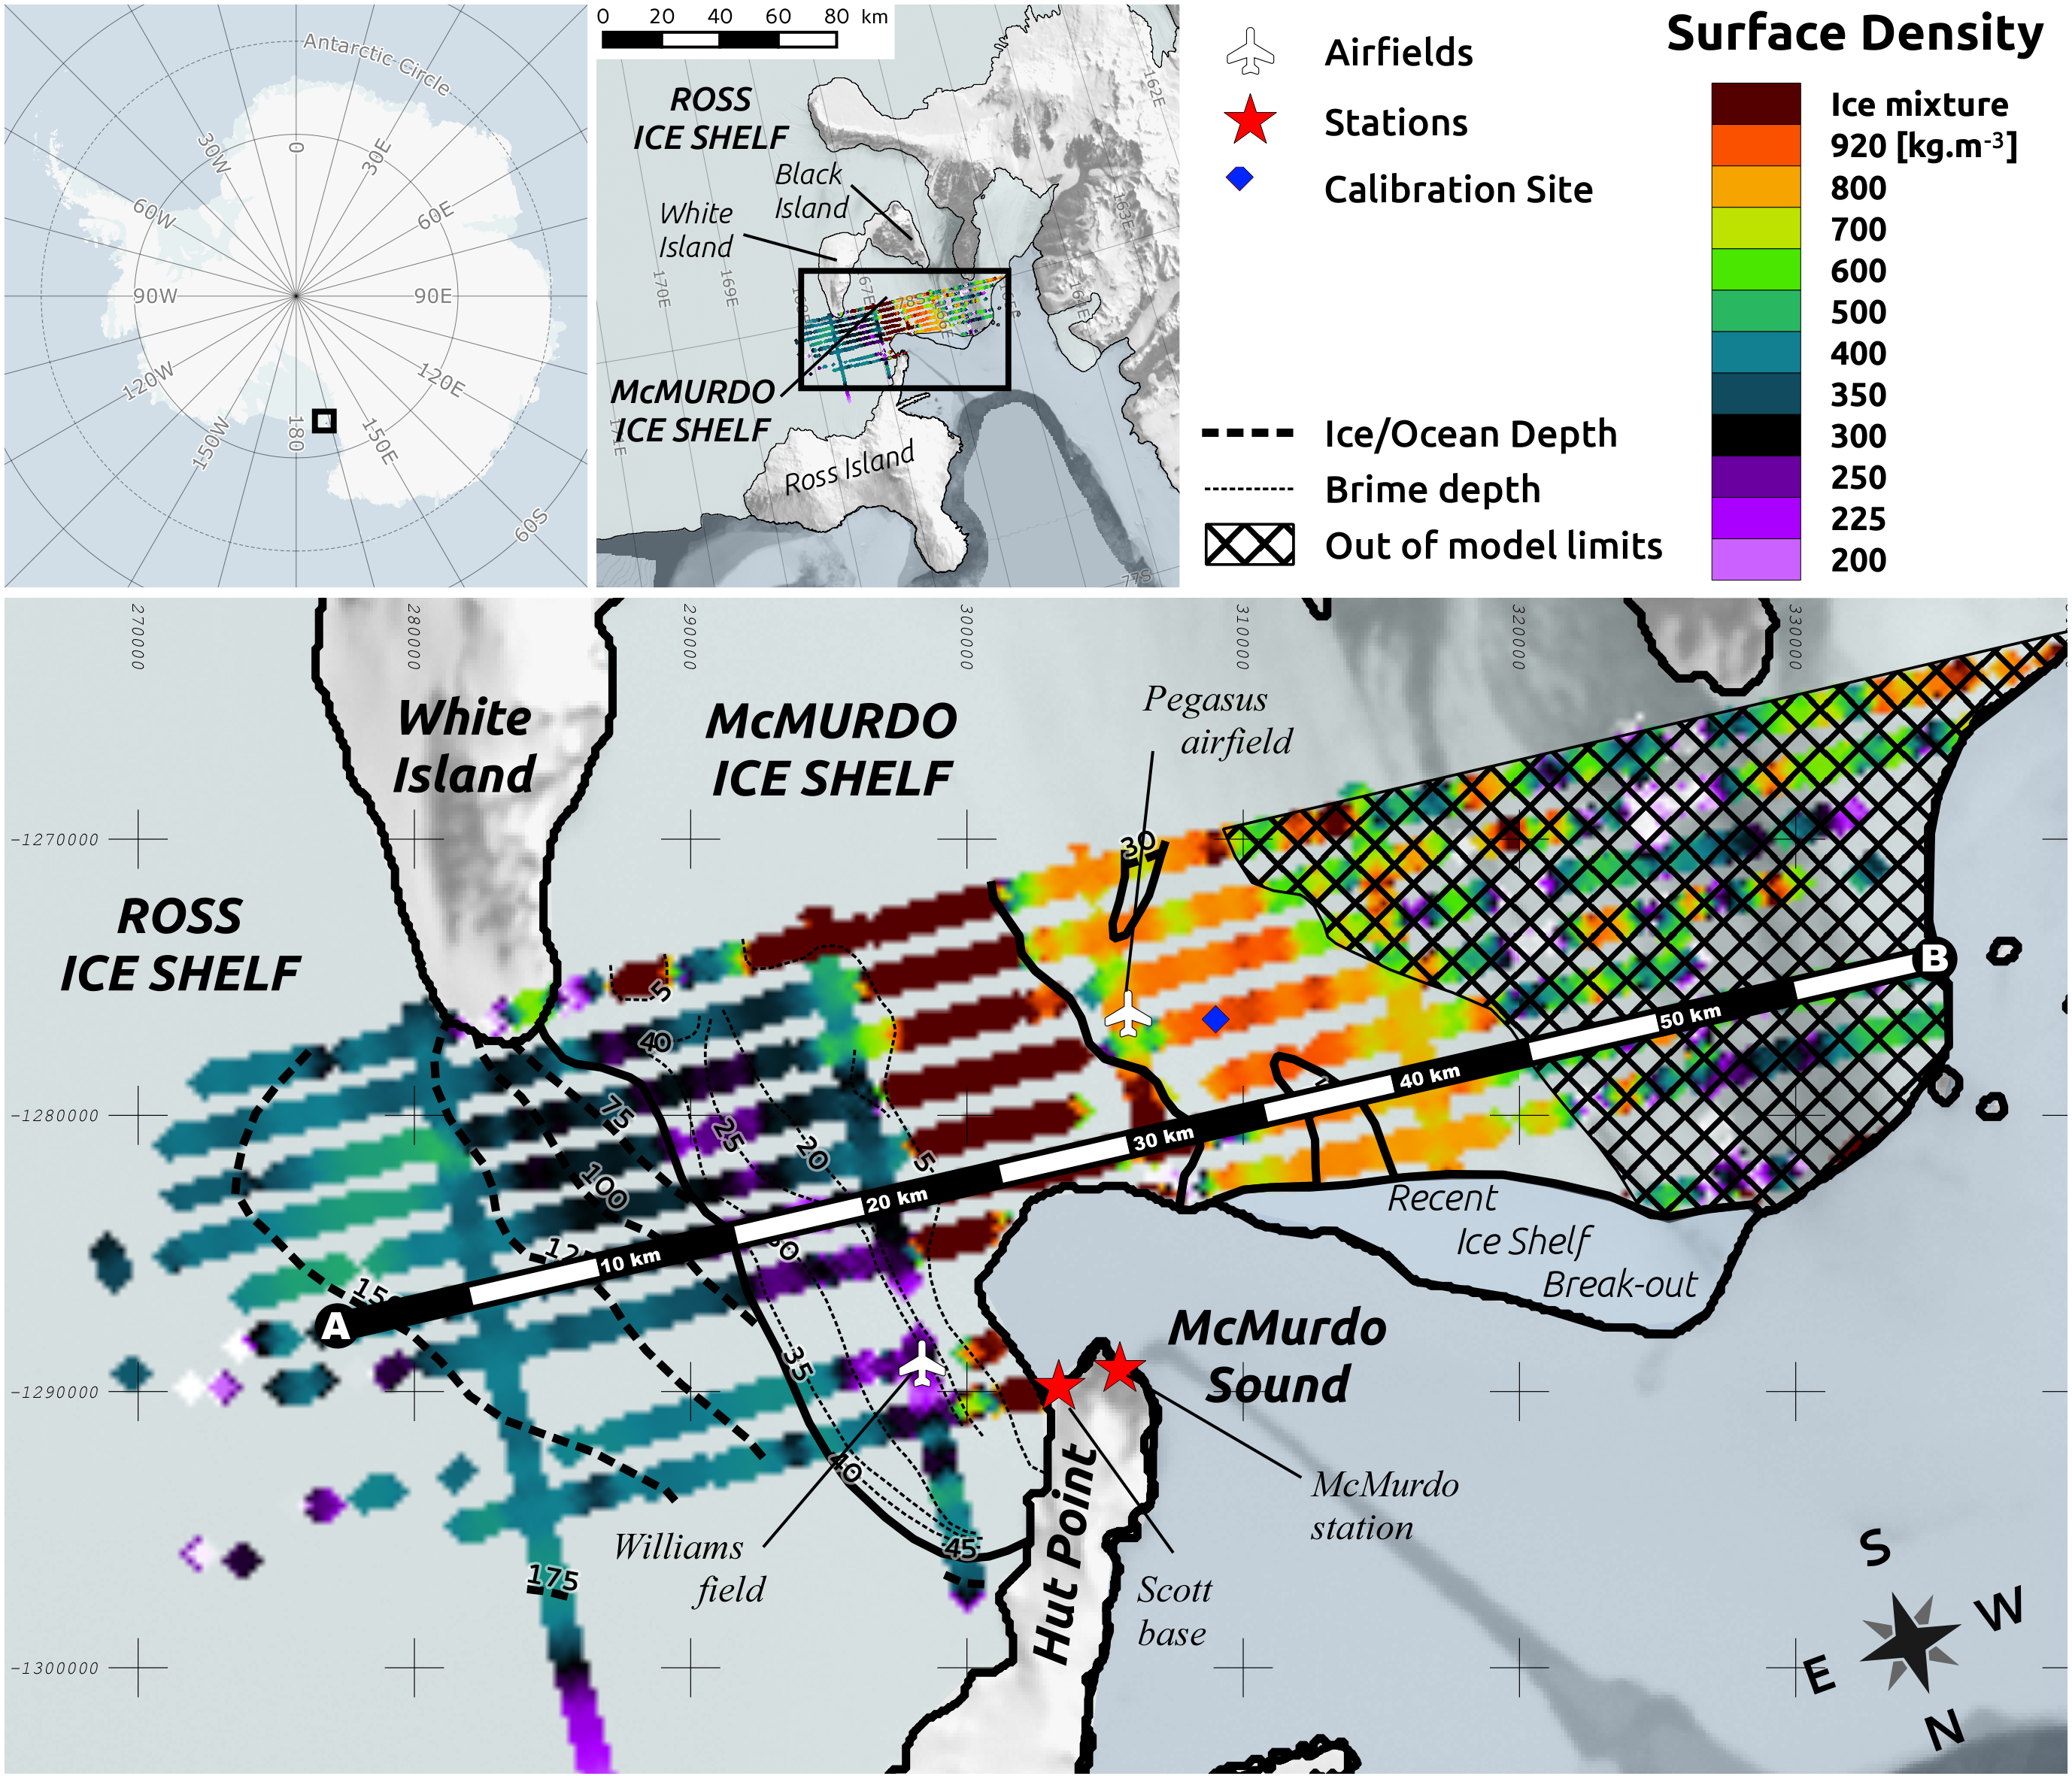
\includegraphics[width=\textwidth]{fig1}
 \caption{\textbf{(Top)} Continental and regional maps illustrating the geographic context of McMurdo Ice Shelf (MIS). \textbf{(Bottom)} Surface densities inverted from RSR-derived permittivities (Fig. S6) and as flown during the 2011-2012 HiCARS2 airborne campaign. "Ice mixtures" indicates a contaminated ice (possibly with liquid water) in the near-surface (down to 5-10m). Ice/ocean interface and brine depths from Fig. \ref{figure_3} are superimposed. The AB segment locates the 60-km long profiles on Fig. \ref{figure_2}.}
  \label{figure_1}
 \end{figure}

% Suggest moving the bottom panel to the top to match the order used in the text and also to give context to the other four panels.
\begin{figure}
 \noindent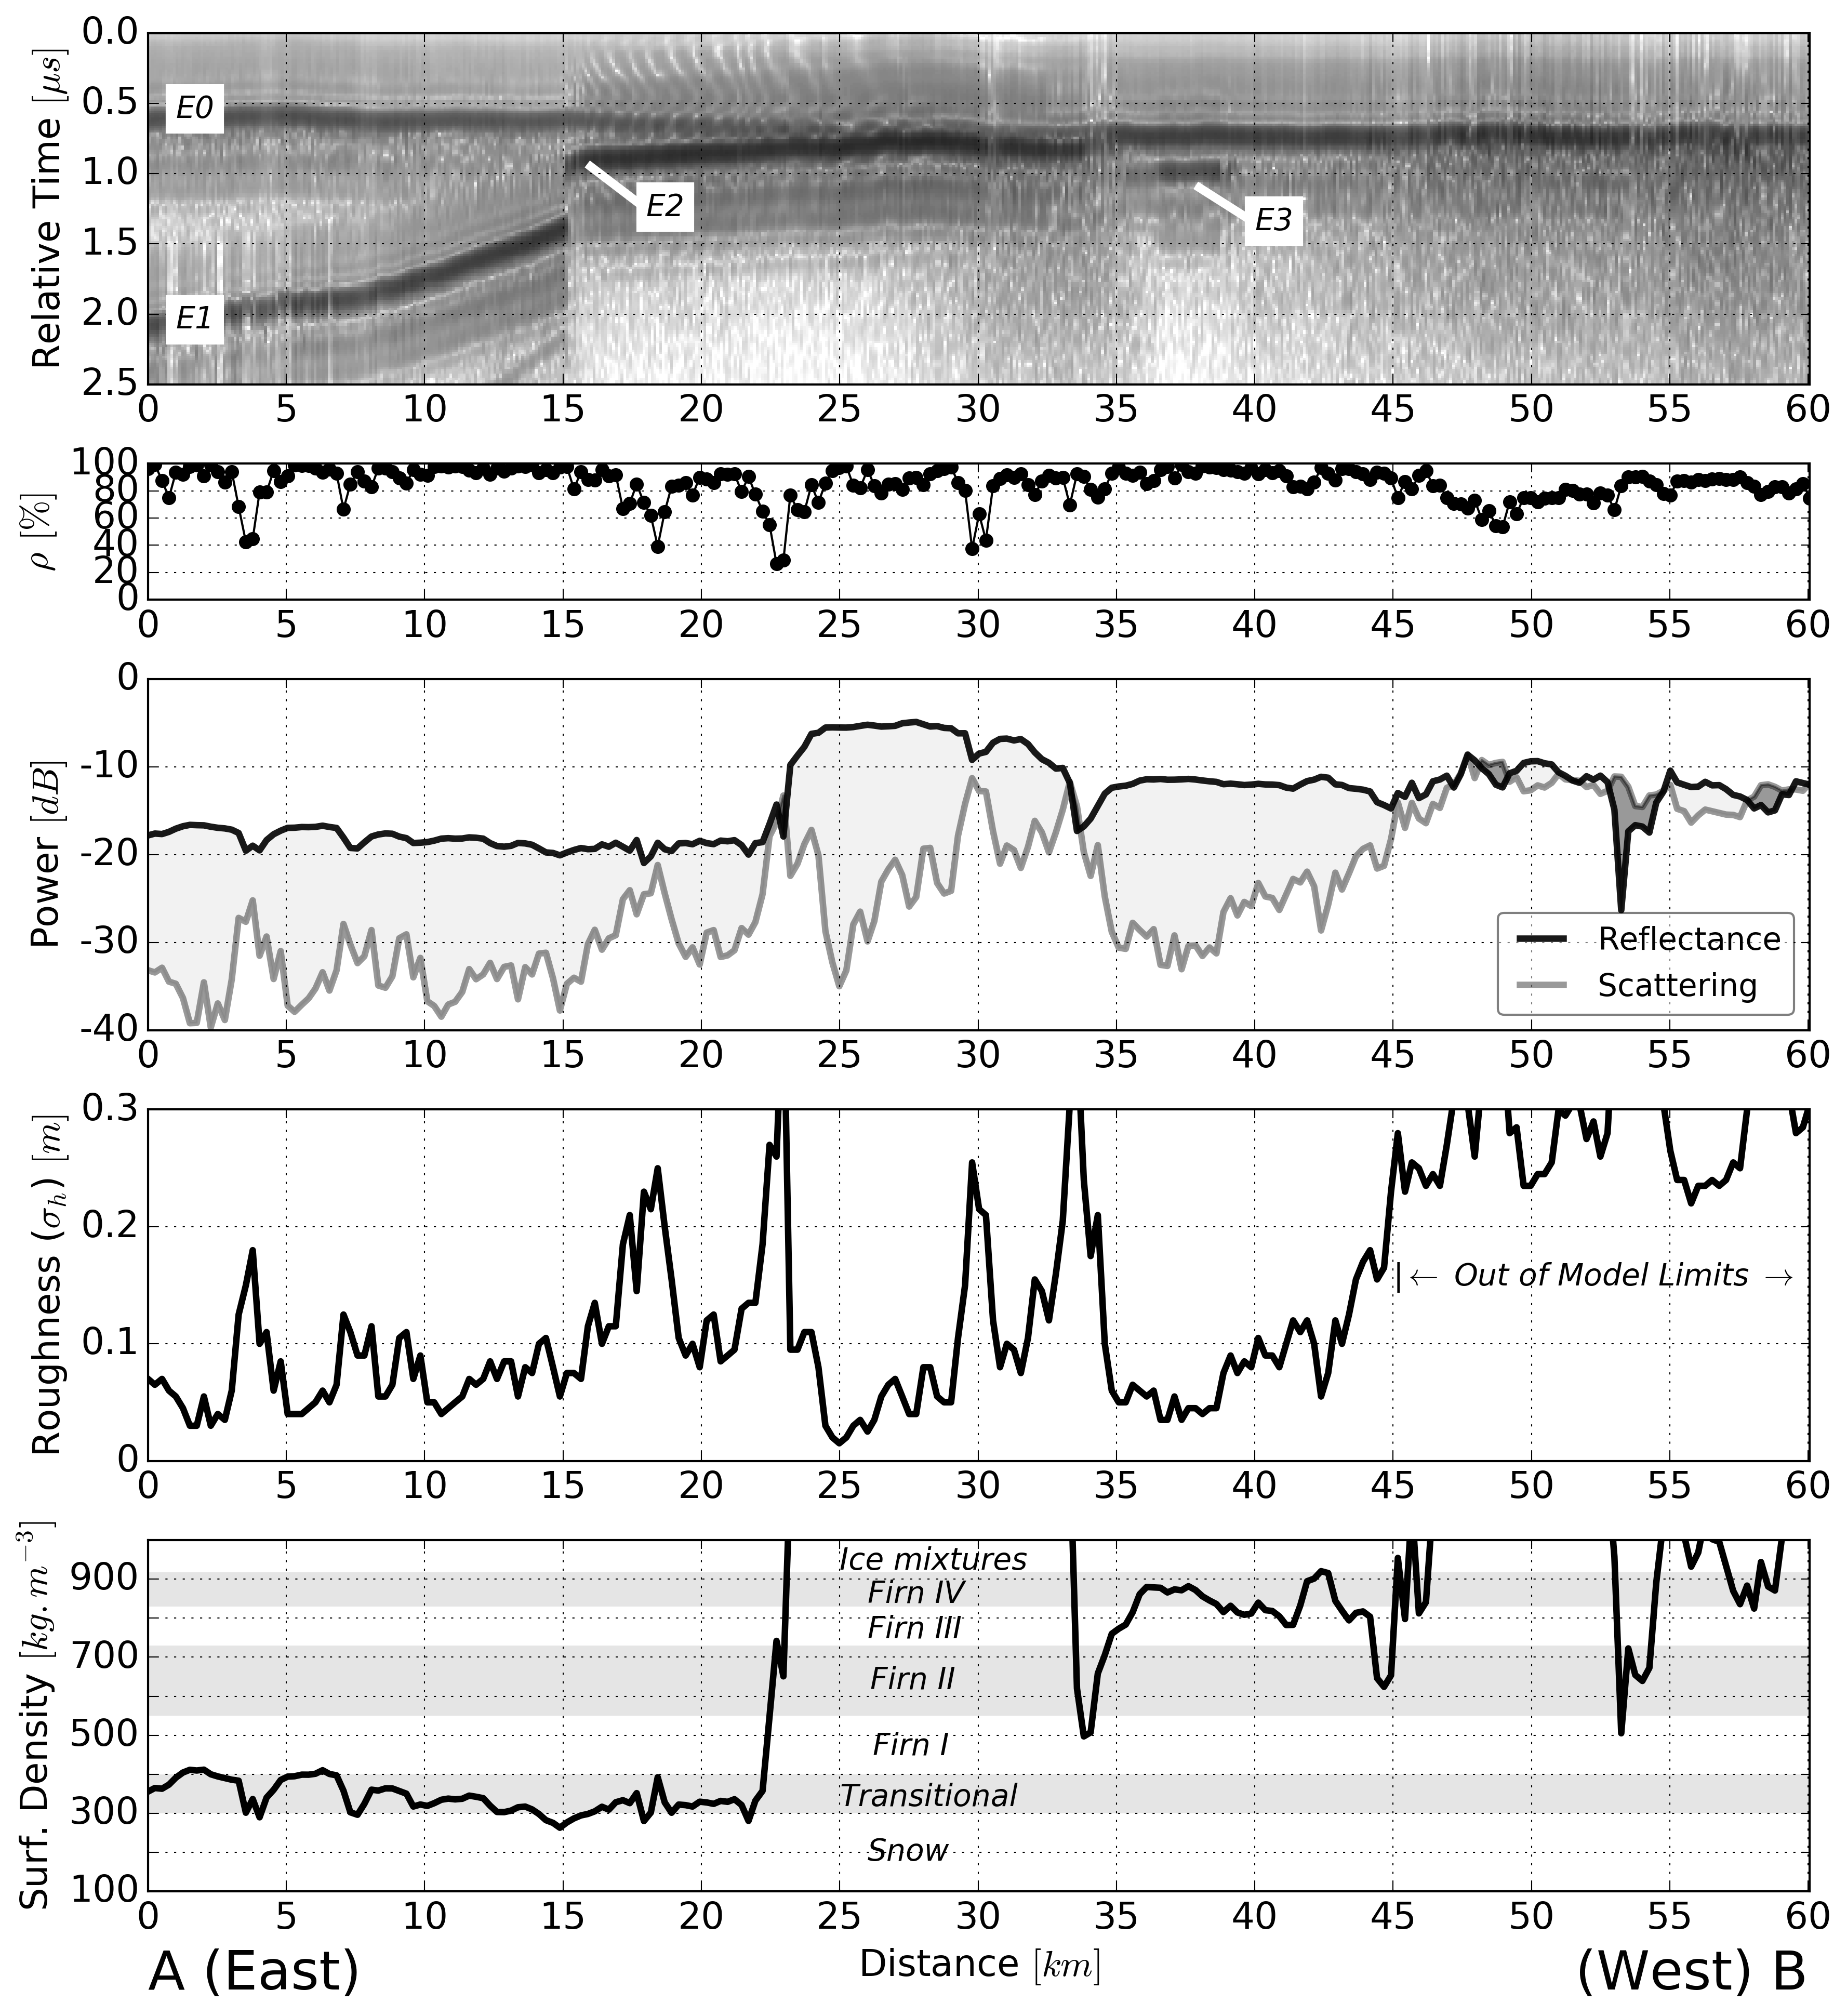
\includegraphics[width=\textwidth]{fig2}
 \caption{Deep and near-surface properties retrieved by radar along segment AB located on Fig. \ref{figure_1}. The top box is the HiCARS2 radargram. E0 labels the surface echo (first return), E1 and E3 represent the ice/ocean interface, E2 is the brine layer. The four bottom boxes are parameters derived from the RSR: correlation coefficient of the statistical fit, reflectance/scattering components, surface root mean square roughness, and surface density, respectively. }
 \label{figure_2}
 \end{figure}


\begin{figure}
 \noindent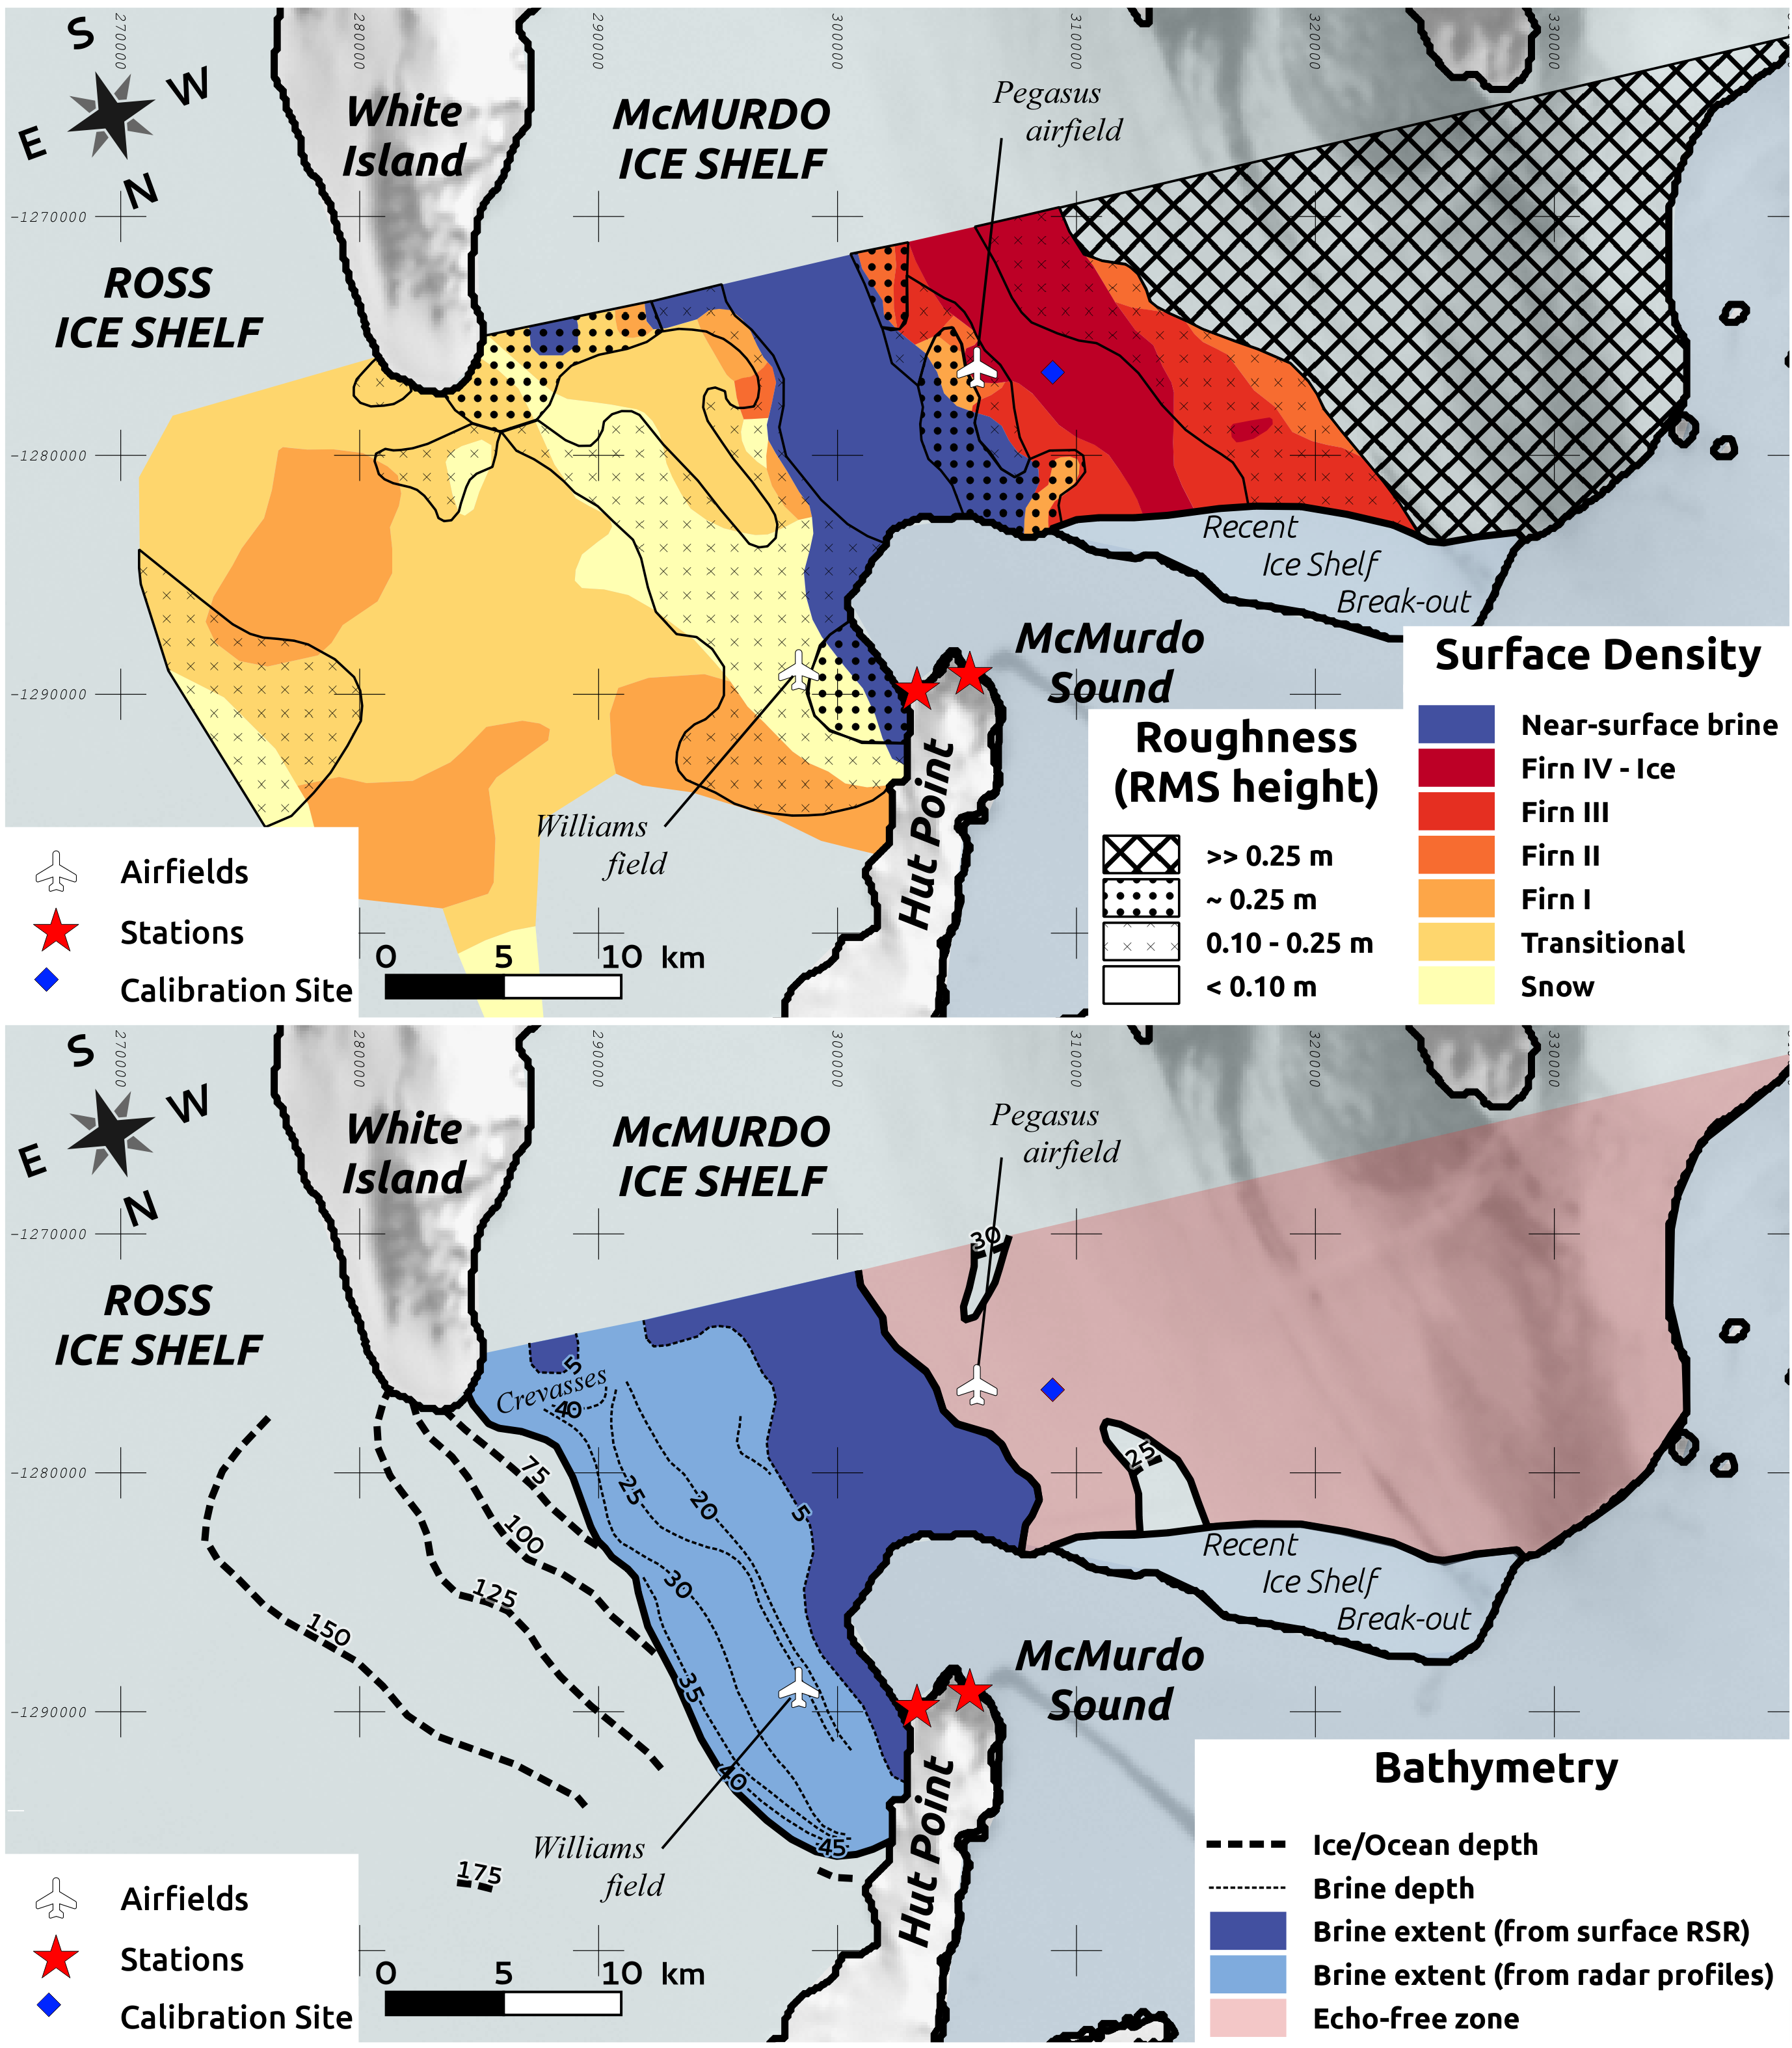
\includegraphics[width=\textwidth]{fig3}
 \caption{\textbf{(Top)} Surface property classification in terms of the RSR-derived roughness and surface density. Snow ($<$~300~kg.m$^{-3}$), snow-firn transition (300-400~kg.m$^{-3}$), firn~I (400-550~kg.m$^{-3}$), firn~II (550-730~kg.m$^{-3}$), firn~III (730-830~kg.m$^{-3}$), and firn~IV-ice (830-917~kg.m$^{-3}$) are the different compaction phases of dry-snow/firn \citep{Cuffey-2010-ID819}. \textbf{(Bottom)} EFZ extent and depth of the brine and ice/ocean interface from radar profile analysis. Depths are given with an uncertainty of $\pm$5-6~m. The RSR-detected brine layer depth is within the radar vertical resolution (5-10~m)}
 \label{figure_3}
 \end{figure}


\begin{figure}
 \noindent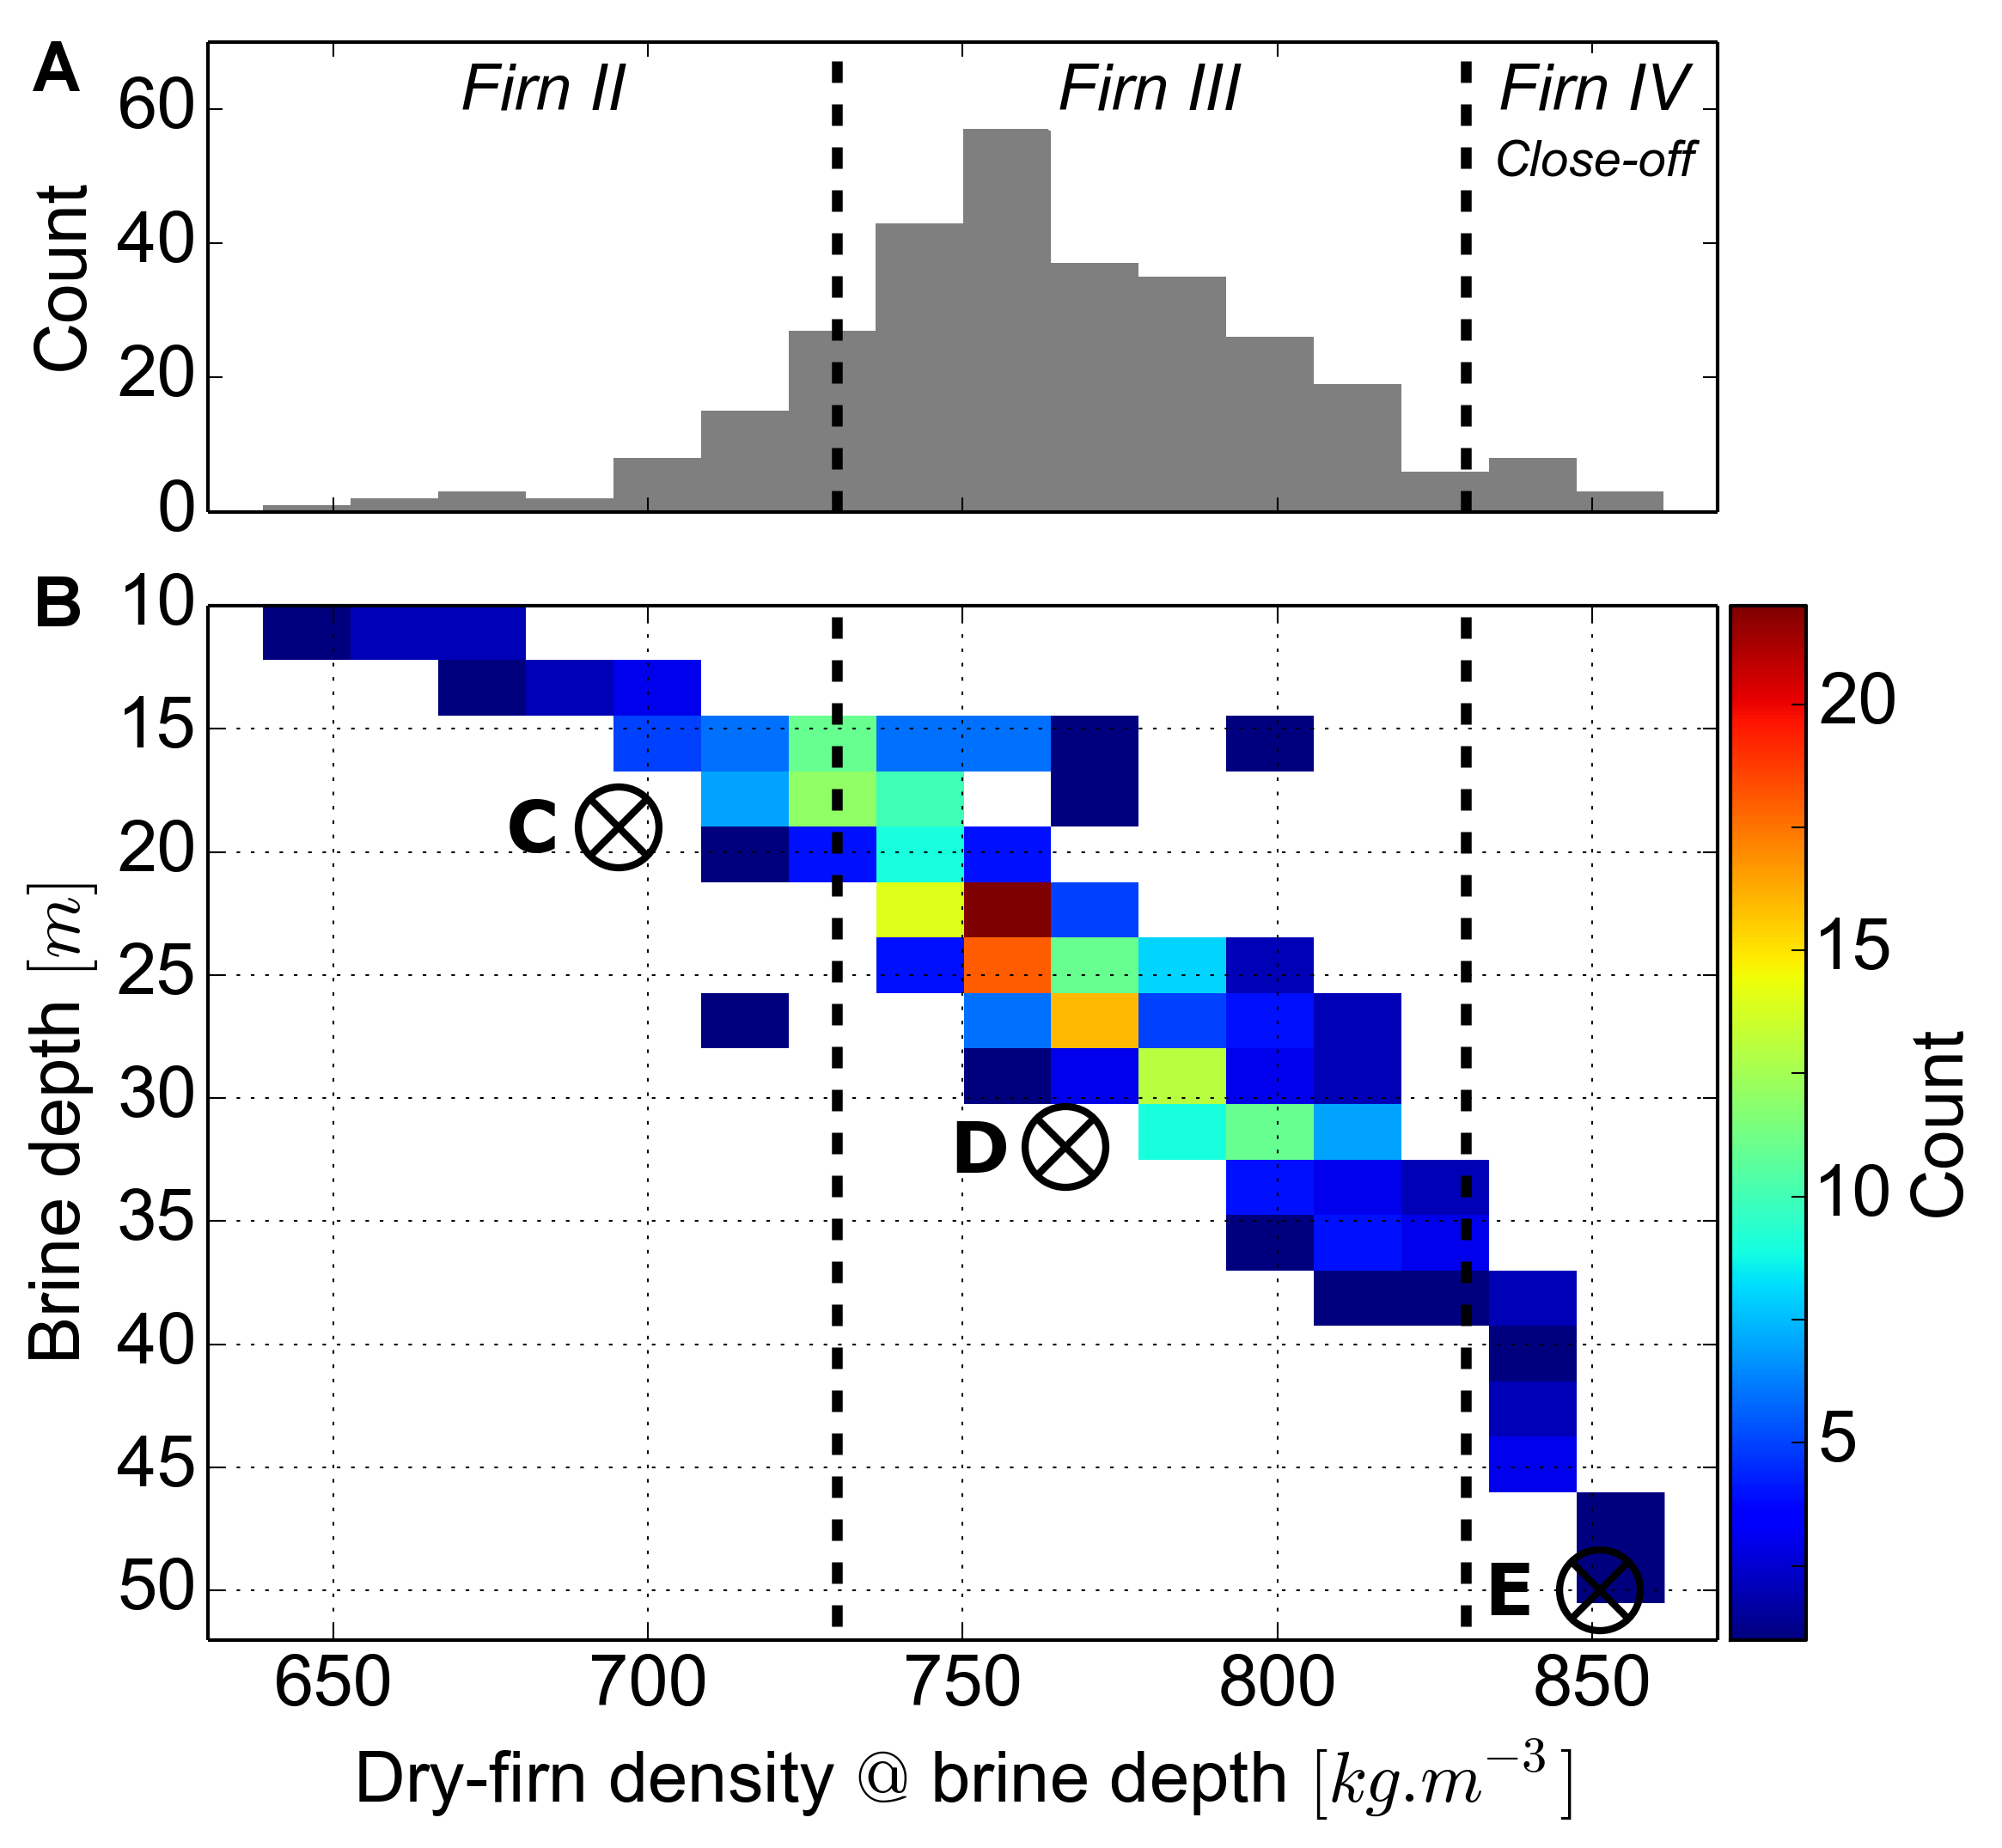
\includegraphics[width=\textwidth]{fig4}
 \caption{\textbf{(A)} Distribution of the equivalent dry-firn density estimated at depth to the top of the brine layer. Firn-III extends from 730~kg.m$^{-3}$ to 830~kg.m$^{-3}$. \textbf{(B)} Same as above broken down with respect to brine depth. The black crossed circles indicate measurements from the ice cores C, D, and E reported by \citet{Kovacs-1982-ID701} just above the brine layer and in the vicinity of Williams field in 1977.}
 \label{figure_4}
 \end{figure}

\end{document}